\jxhj{%教学后记
	}
\skrq{%授课日期
	2017年11月16日 4-5节}
\ktmq{%课题名称
	 岛屿型腔加工}
\jxmb{%教学目标,每行前面要加 \item
	\item 掌握岛屿型腔加工的下刀方式;
    \item 掌握岛屿槽去残料的方式;
    \item 会用G91螺线下刀及Z向分层;
    \item 会编写岛屿型腔的程序。}
\jxzd{%教学重点,每行前面要加 \item
	\item 编写岛屿型腔的程序;
	\item G91螺线下刀及Z向分层。 }
\jxnd{%教学难点,每行前面要加 \item
	\item 编写岛屿型腔的程序。 }
\jjff{%教学方法
	通过讲述、举例、演示法来说明;}

\makeshouye %制作教案首页

%%%%教学内容
\subsection{组织教学}
\begin{enumerate}[\hspace{2em}1、]
	\item 集中学生注意力;
	\item 清查学生人数;
	\item 维持课堂纪律;
\end{enumerate}

\subsection{复习导入及主要内容}
\begin{enumerate}[1、]
\item 刀具的选择;
\item 下刀方式;
\item 斜线下刀;
\item 去残料方式;
\item 方槽铣削加工实例。
\end{enumerate}

\subsection{教学内容及过程}
\subsubsection{加工实例}
实例:用数控铣完成如图10-1所示零件的加式工。零件材料为45号钢,毛坯为\diameter 110×35mm。按图样要求完成零件基点及辅助点的计算,设定工件坐标系,制定正确的工艺方案(包括定位、夹紧方案和工艺路线),选择合理的刀具和切削工艺参数,编制数控加工程序。

\begin{figure}[h]
	\centering
	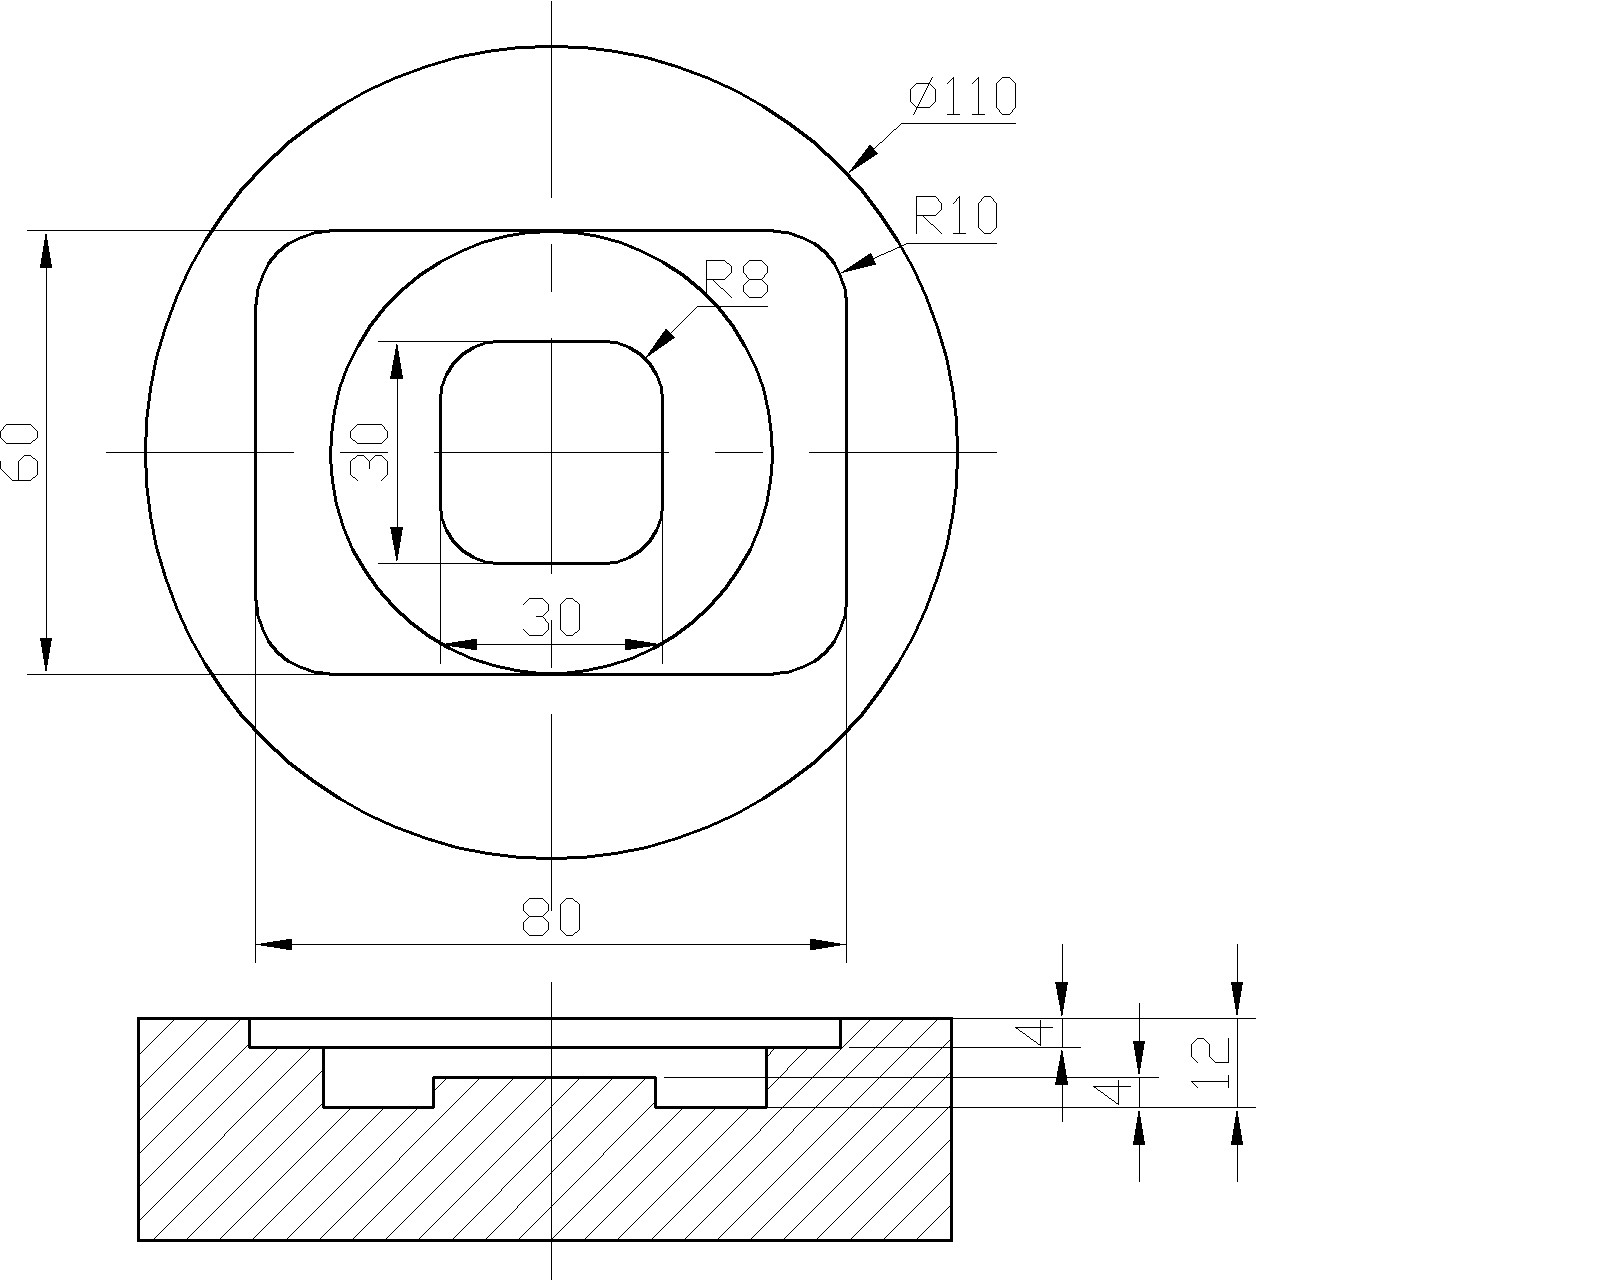
\includegraphics[width=0.8\linewidth,trim=0 0 150  0,clip]{data/image/19-1.jpg}
	\caption{岛屿型腔加工}
	\label{fig:19-1}
\end{figure}

\subsubsection{刀具选择及工艺路线}
1、工艺分析

此工件毛坯加工完成,只要进行槽的加工,且所有精度一样,没有其它要求。零件的装夹采用平口钳装夹。将工件坐标系G54建立在工件上表面、零件的对称中心。针对零件图样要求给出加工工序为:

(1)用Z向分两层加工φ60*8的槽

(2)加工中间的岛屿

(3)用刀补加工长方形的槽。

2、刀具的选择

最小内凹圆弧半径为R10,且岛屿间的最小间距约为12mm,故粗加工用φ10的立铣刀。精加工用φ10的立铣刀。

3、切削参数的选择

粗加工   S500   F100

精加工   S800   F80

粗加工补 D1=5.5

精加工补 D2=(计算所得)

4、加工路径:

(1)螺旋下刀:

为使岛屿共用一个下刀,用R24的圆弧螺旋下刀,如图所示:

\begin{figure}[h]
    \centering
    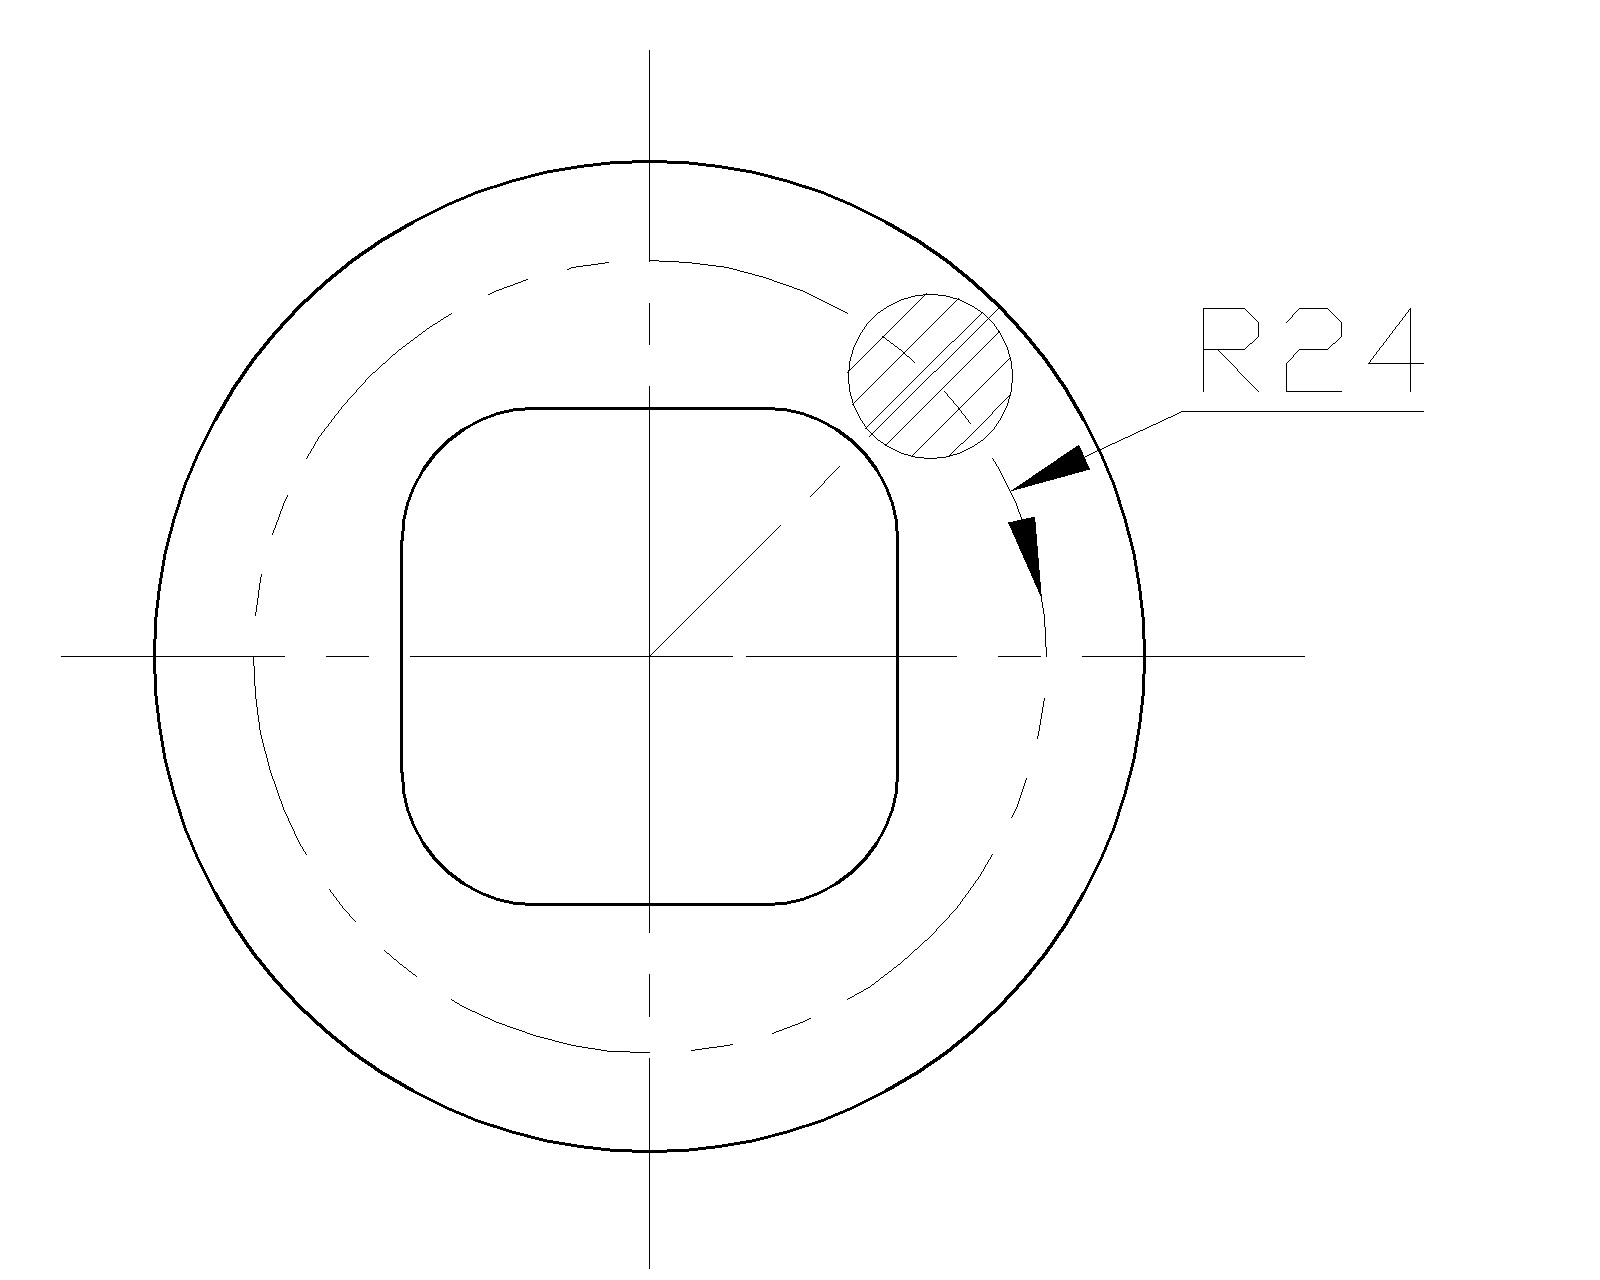
\includegraphics[width=0.6\linewidth,trim=0 0 120  0,clip]{data/image/19-2.jpg}
    \caption{}
    \label{fig:19-2}
\end{figure}

(2)圆形\diameter 60的槽:

路径如图所示:R18、R8

\begin{figure}[h]
    \centering
    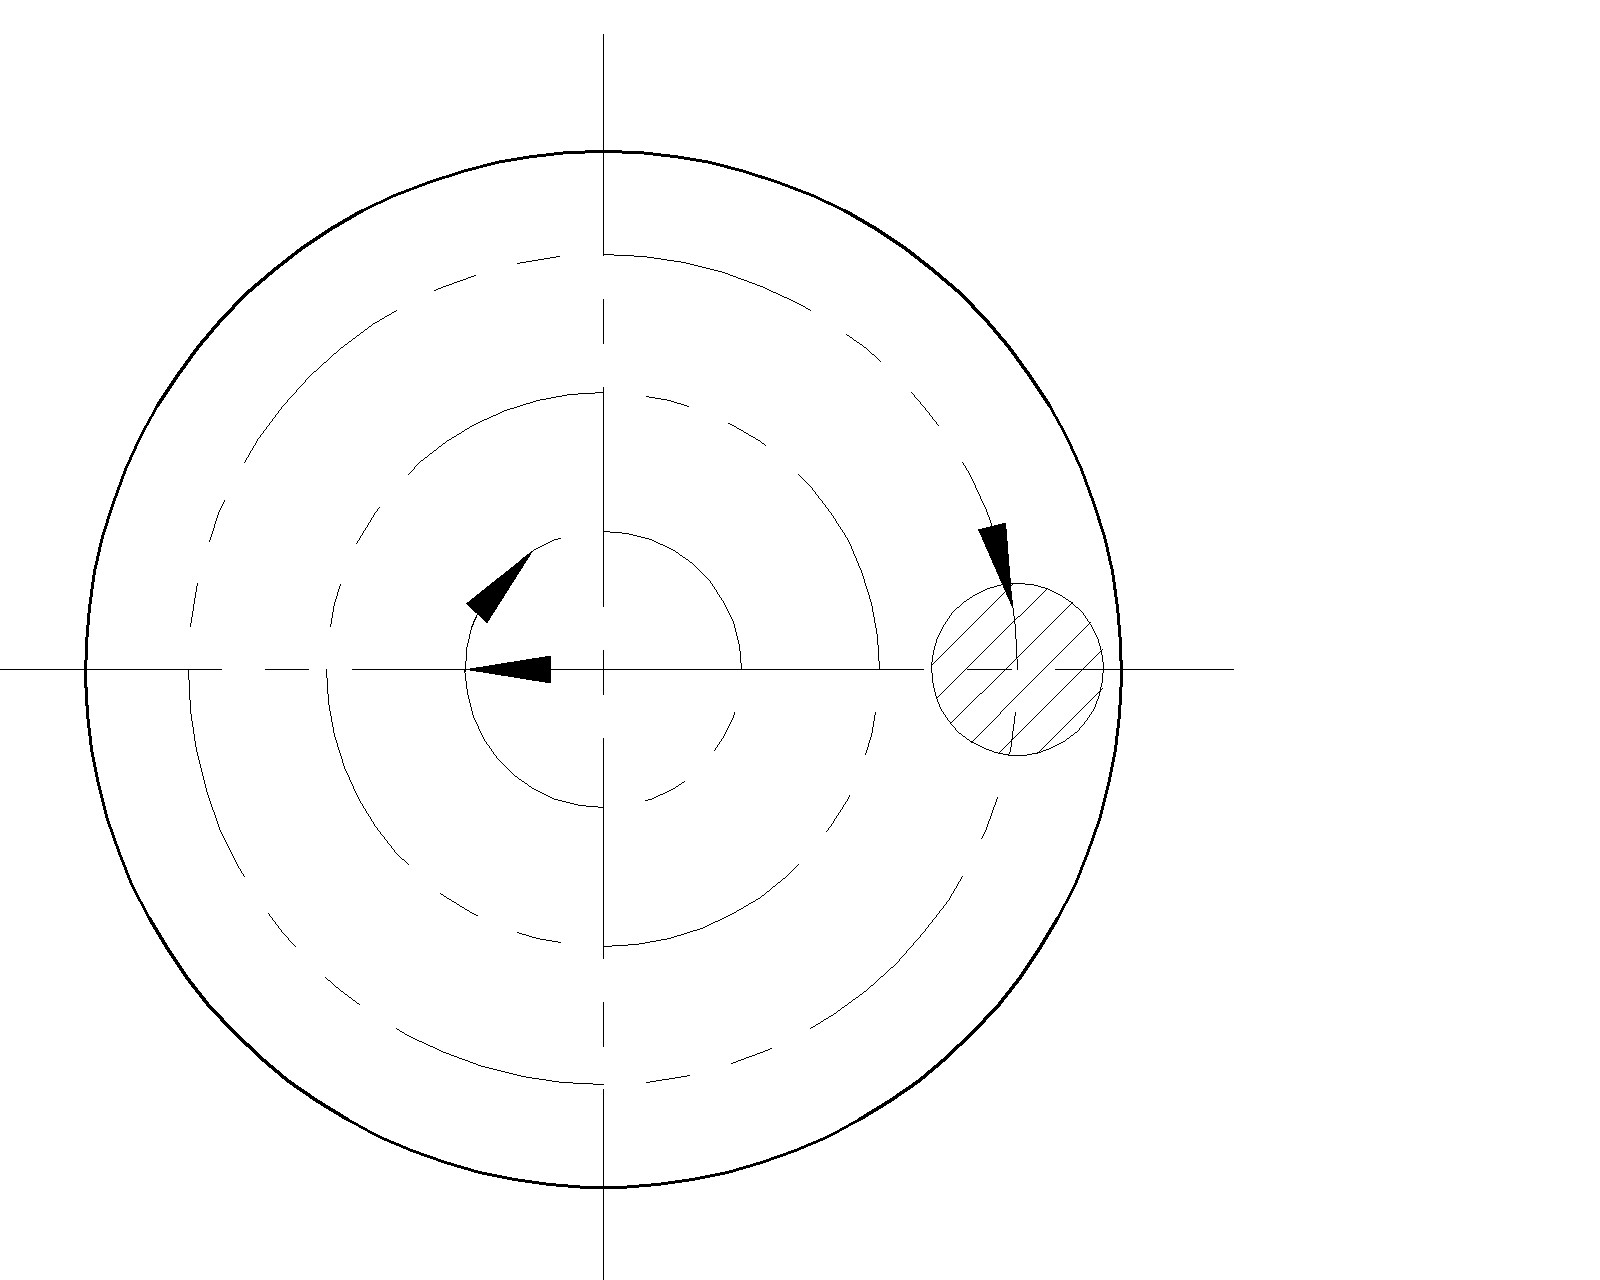
\includegraphics[width=0.6\linewidth,trim=0 0 130  0,clip]{data/image/19-3.jpg}
    \caption{}
    \label{fig:19-3}
\end{figure}

(3)圆形精加工路径

如图所示,要注意不能有干涉,采用顺铣。

\begin{figure}[h]
    \centering
    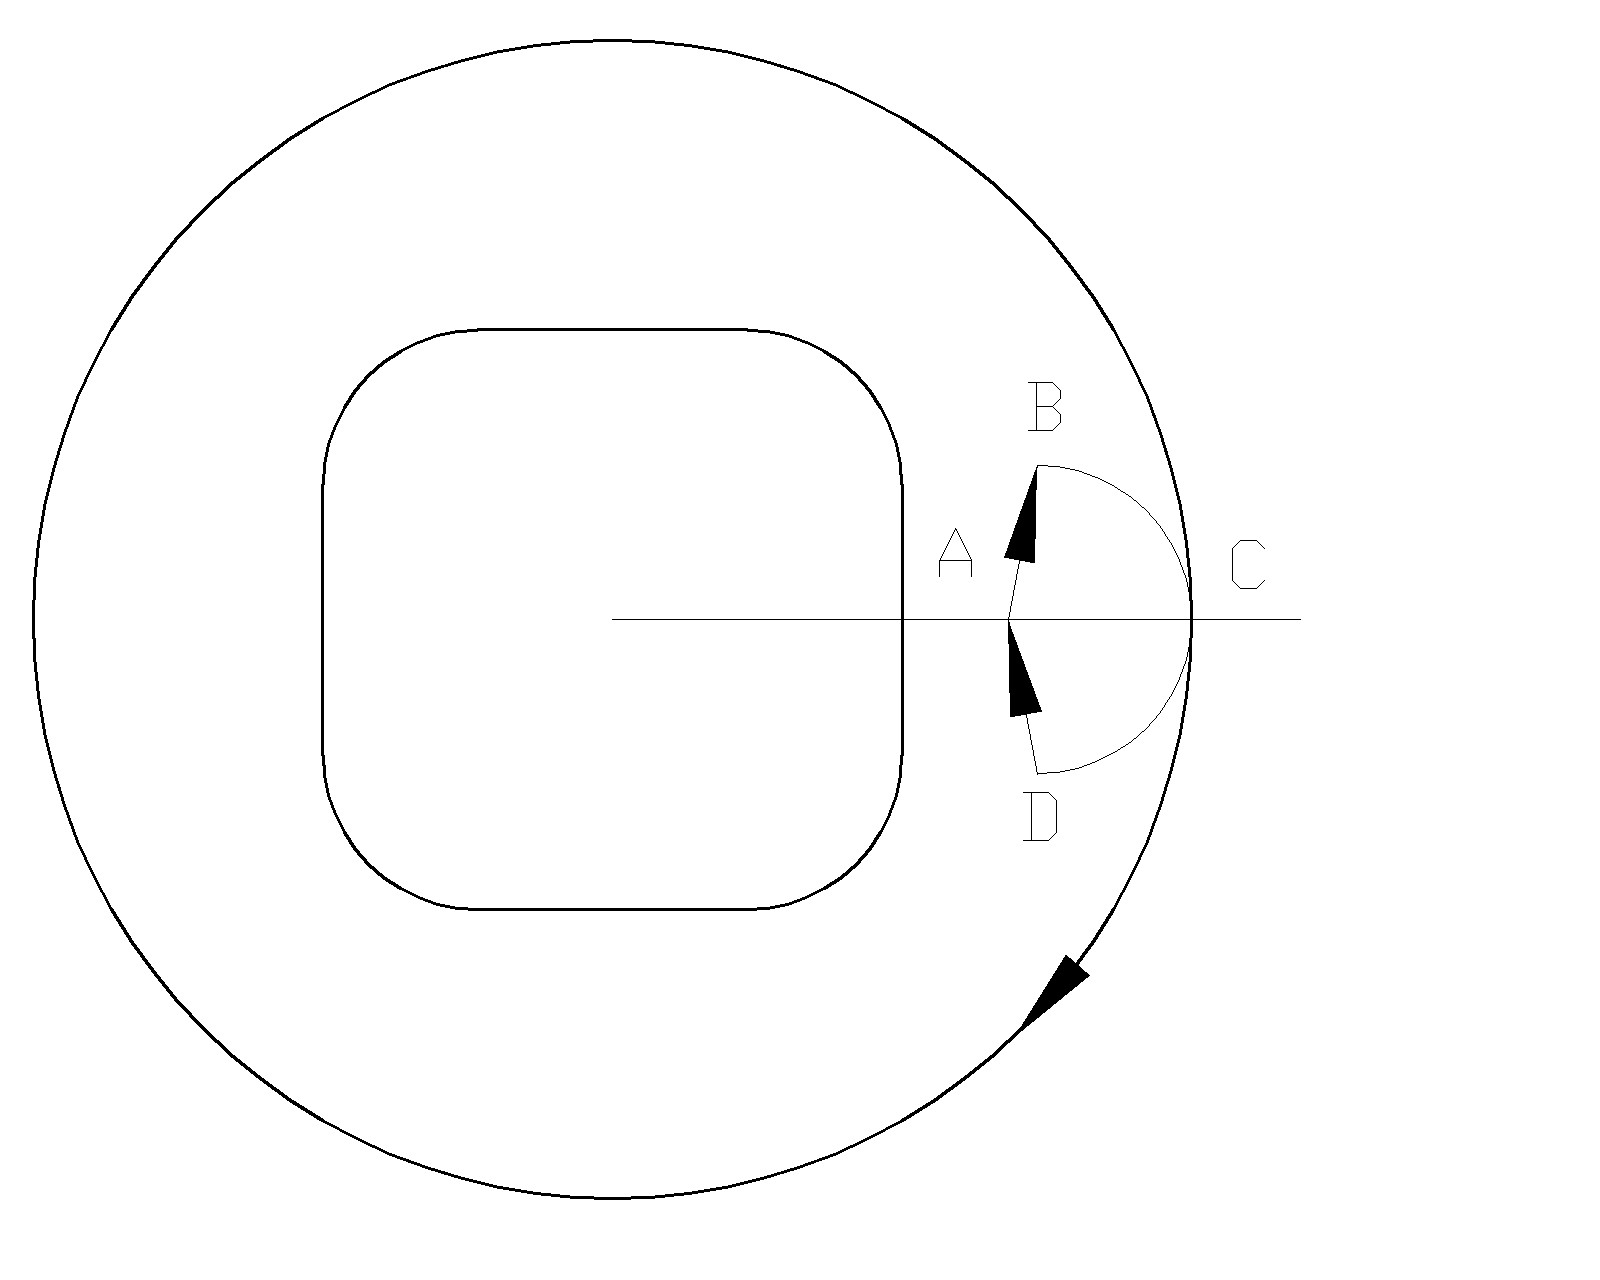
\includegraphics[width=0.6\linewidth,trim=0 0 130  0,clip]{data/image/19-4.jpg}
    \caption{}
    \label{fig:19-4}
    坐标:A(20.5,0)B(22,8)C(30,0)D(22,-8)
\end{figure}


(4)岛屿精加工路径

同上,如图所示:
\begin{figure}[h]
    \centering
    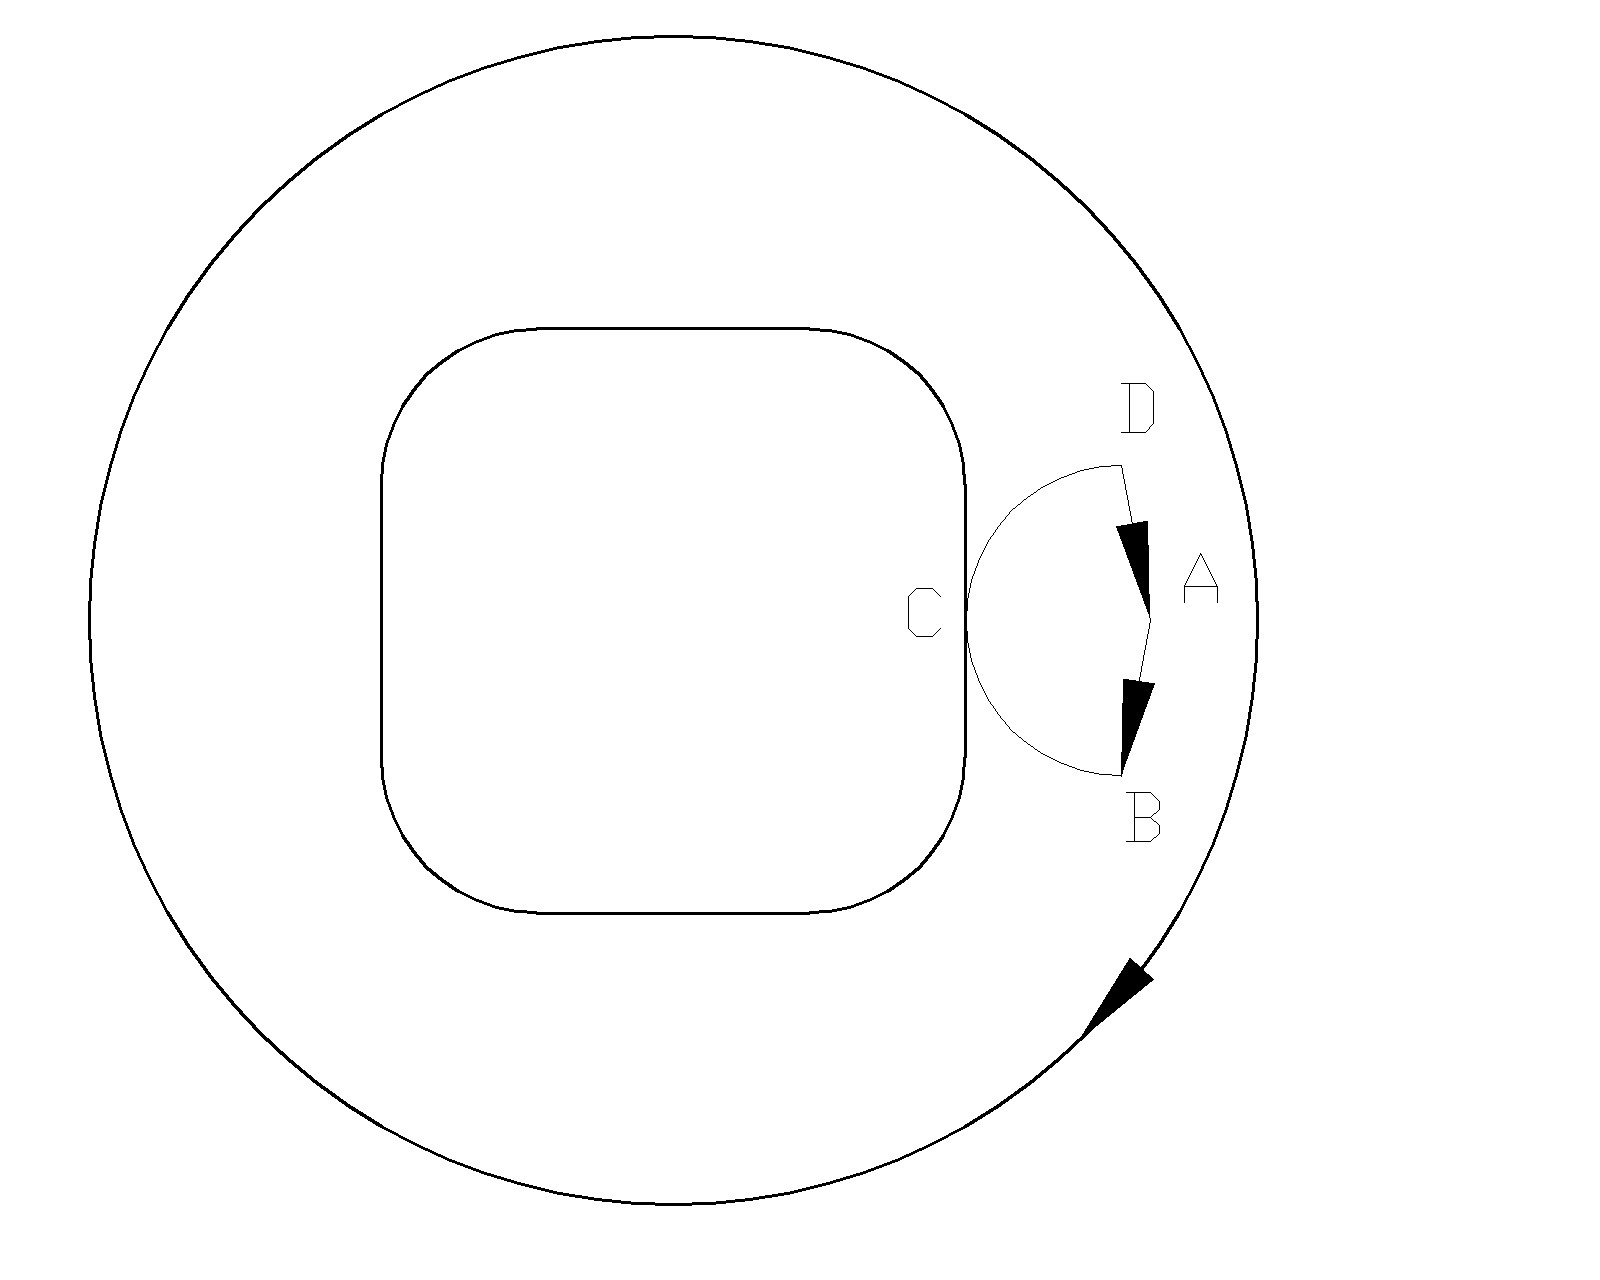
\includegraphics[width=0.6\linewidth,trim=0 0 130  0,clip]{data/image/19-5.jpg}
    \caption{}
    \label{fig:19-5}
    坐标A(24.5,0)B(23,-8)C(15,0)D(23,8)
\end{figure}



(5)方形精加工路径

如图所示:
\begin{figure}[h]
    \centering
    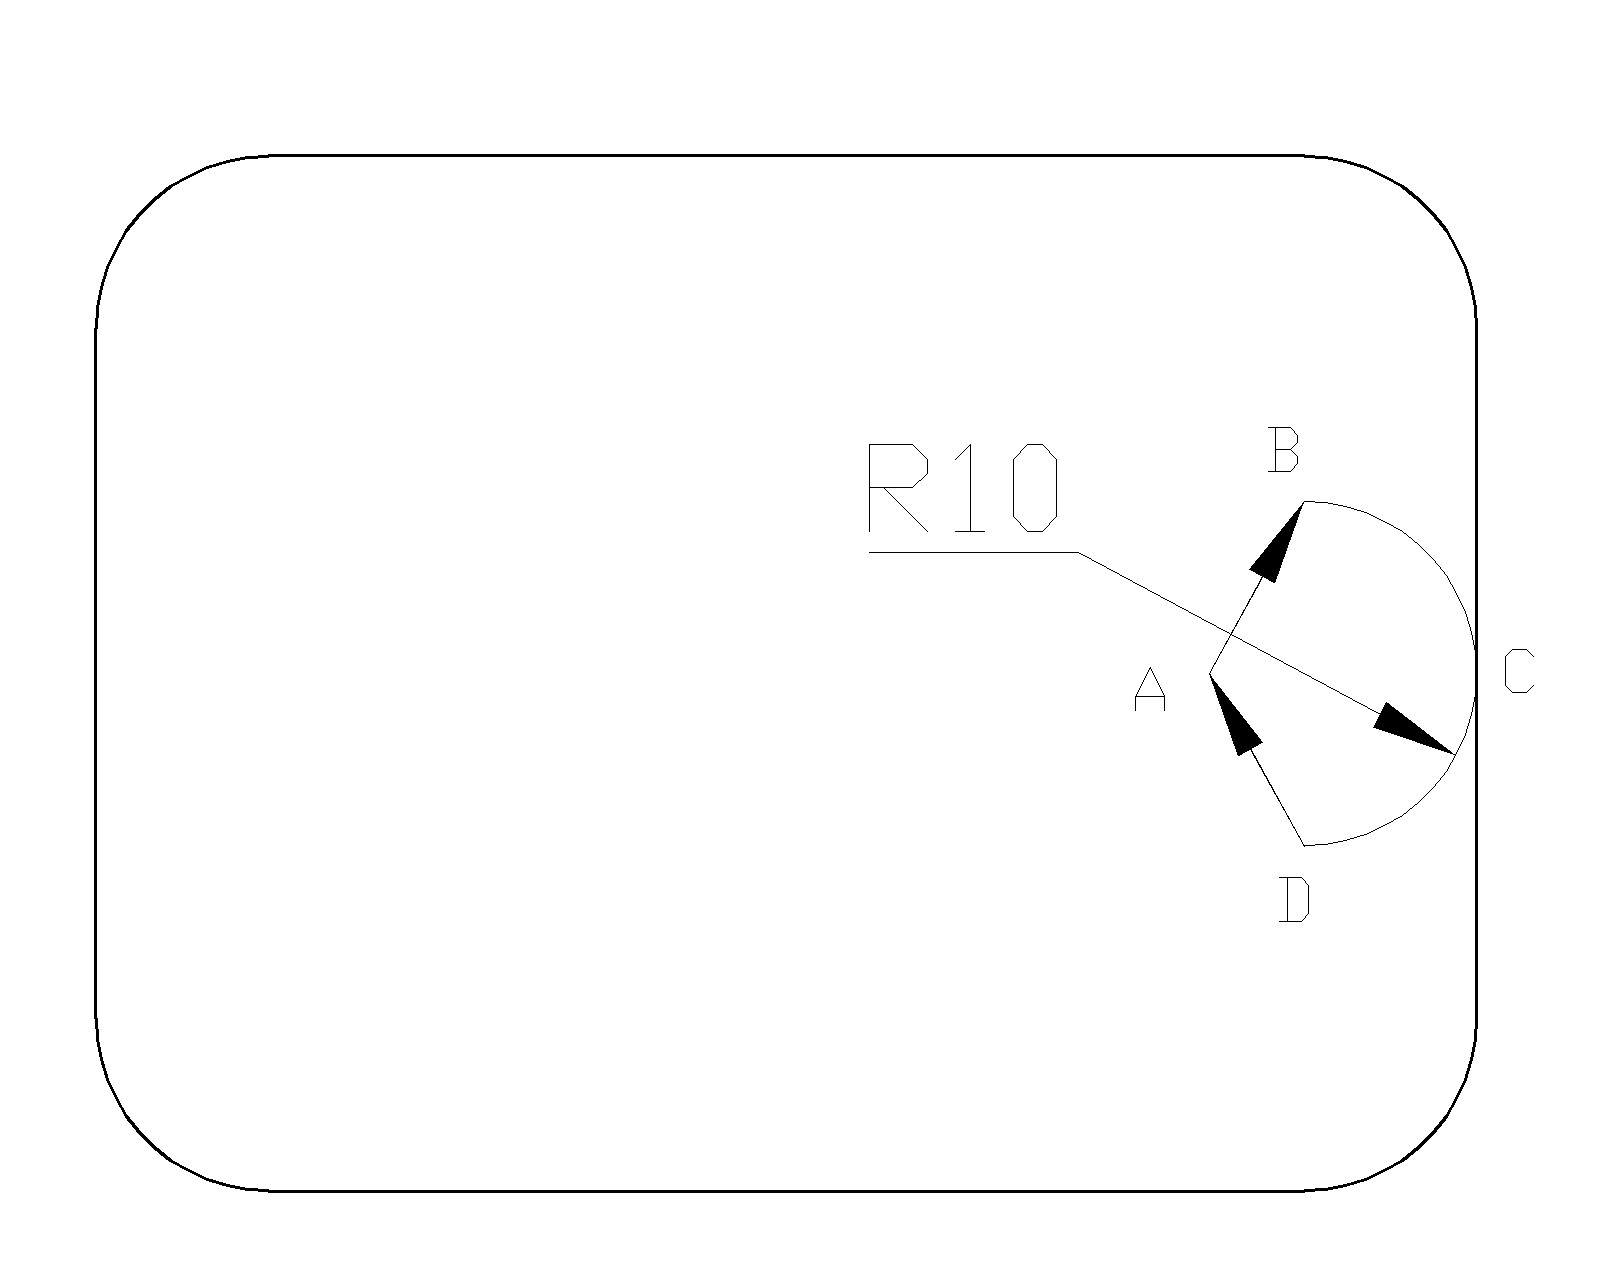
\includegraphics[width=0.6\linewidth,trim=0 0 130  0,clip]{data/image/19-6.jpg}
    \caption{}
    \label{fig:19-6}
    坐标 A(24.5,0)B(30,10)C(40,0)D(30,-10)
\end{figure}

5、Fanuc上的参考程序:
\begin{lstlisting}
O0001;(粗加工主程序)
G54 G17 G40 G49 G90;
M3 S500;
G0 Z30.0;
X24.0 Y0;
Z2.0;
G1 Z0 F100.0;
M98 P20002;    圆形槽
G2 X24.0 Y0 Z-12.0 I-24 J0;   
G2 I-24.0 J0;
G1 X20.5 Y0;    定位到圆形槽A点
D1 M98 P3;     粗加工圆 
G1 X24.5 Y0;    定位到岛屿路径A点
D1 M98 P4;     粗加工岛屿      
G1 Z-4.0;
G1 X27.0 Y0    加工方形槽
Y-17.0
X-27.0
Y17.0
X27.0 
Y0
X24.5 Y0    
D1 M98 P5;   粗加工方形槽
G0 Z30.0;
M5;
M30;
\end{lstlisting}

\begin{lstlisting}
O0002;            粗加工圆形槽
G91 G02 X0 Y0 Z-4.0 I-24.0 J0
G90 G02 I-24.0 J0
G1X-8.0 Y0
G2 I8.0 J0
G1 X-16.0 Y0
G2 I16.0 J0
G1 X20.5 Y0
D1 M98 P3
G1 X24.0 Y0
M99
\end{lstlisting}

\begin{lstlisting}
O0003        圆形槽轮廓子程序
G42 G1 X22.0 Y8.0
G2 X30.0 Y0 R8.0
G2 I-30.0 J0
G2 X22.0 Y-8.0 R8.0
G40 G1 X20.5 Y0
M99
\end{lstlisting}

\begin{lstlisting}
O0004      岛屿轮廓子程序
G42 G1 X23.0 Y-8.0 
G2 X15.0 Y0 R8.0
G1 Y7.0
G3 X7.0 Y15.0 R8.0
G1 X-7.0 
G3 X-15.0 Y7.0 R8.0
G1 Y-7.0 
G3 X-7.0 Y-15.0 R8.0
G1 X7.0 
G3 X15.0 Y-7.0 R8.0
G1 Y0
G2 X23.0 Y8.0 R8.0
G40 G1 X24.5 Y0
M99
\end{lstlisting}

\begin{lstlisting}
O0005        方形槽轮廓子程序
G42 G1 X30.0 Y10.0
G2 X40.0 Y0 R10.0
G1 Y-20.0 
G2 X30.0 Y-30.0 R10.0
G1 X-30.0 
G2 X-40.0 Y-20.0 R10.0
G1 Y20.0 
G2 X-30.0 Y30.0 R10.0
G1 X30.0 
G2 X40.0 Y20.0 R10.0
G1 Y0 
G2 X30.0 Y-10.0 R10.0
G40 G1 X24.5 Y0
M99
\end{lstlisting}

\begin{lstlisting}
O0006       精加工子程序
G54 G17 G40 G49 G90 
M3 S800
G0 Z30.0
X20.5 Y0
Z2.0
G1 Z-12.0 F80
D2 M98 P3
G1 X24.5 Y0
D2 M98 P4
G1 Z-4.0
D2 M98 P5
G0 Z30.0
M99
\end{lstlisting}



\subsection{课堂小结}
\begin{enumerate}[1、]
\item 岛屿型腔加工的下刀方式;
\item 岛屿槽去残料的方式;
\item 用G91螺线下刀及Z向分层;
\item 编写岛屿型腔的程序。
\end{enumerate}

\vfill
\subsection{布置作业}
\begin{enumerate}[1、]
	\item 编写上面的程序。
\end{enumerate}
\vfill